\documentclass[class=minimal,border=0pt]{standalone}
\usepackage{tikz}


\begin{document}
	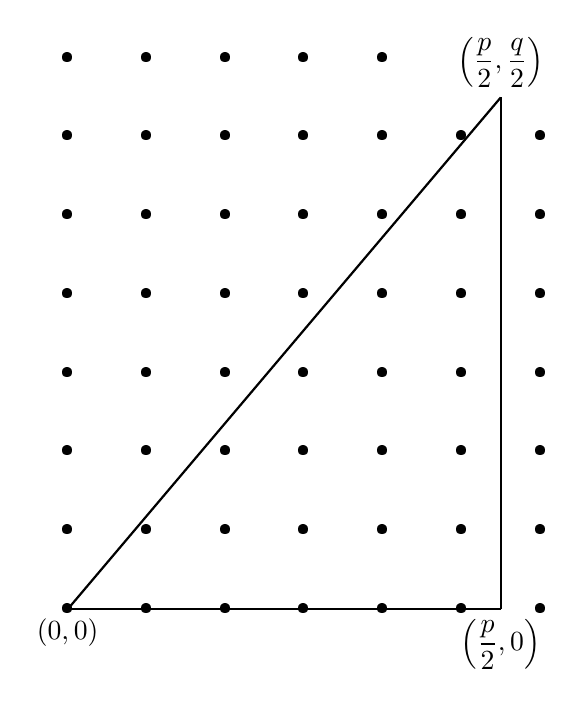
\begin{tikzpicture}
	\draw[thick] (0,0)--(5.5,6.5);
	\draw[thick] (5.5,6.5)--(5.5,0);
	\draw[thick] (0,0)--(5.5,0);
	
	\foreach \Point in {(0,0), (0,1), (0,2), (0,3), (0,4), (0,5), (0,6), (0,7),
		(1,0), (1,1), (1,2), (1,3), (1,4), (1,5), (1,6), (1,7),
		(2,0), (2,1), (2,2), (2,3), (2,4), (2,5), (2,6), (2,7),
		(3,0), (3,1), (3,2), (3,3), (3,4), (3,5), (3,6), (3,7),
		(4,0), (4,1), (4,2), (4,3), (4,4), (4,5), (4,6), (4,7),
		(5,0), (5,1), (5,2), (5,3), (5,4), (5,5), (5,6),
		(6,0), (6,1), (6,2), (6,3), (6,4), (6,5), (6,6)}{
		\node at \Point {\textbullet};
	}
	
	\node [below] at (0,0) {$(0,0)$};
	\node [below] at (5.5,0) {$\displaystyle\left(\frac{p}{2},0\right)$};
	\node [above] at (5.5,6.5) {$\displaystyle\left(\frac{p}{2},\frac{q}{2}\right)$};
	\end{tikzpicture}
\end{document}
